\documentclass[12pt]{report}

\usepackage{style}

\typeMemoire{Diplôme de Licence Professionnelle en Systèmes d'Information et Réseaux Informatiques}
%\optionFormation{Informatique Générale}
\etudiant{Vincent-Béni \textbf{ZOSSOU}}
\titreDuMemoire{ITAJA : Système intégré de gestion d’un commerce}


\anneeScolaire{2016-2017}
%\pdfkeywords={mots clé, du, mémoire, IFRI} 

% Plusieurs encadrants décommenté la ligne suivante
\encadrants{M. Fréjus \textbf{LALEYE}\\ M. Paterne \textbf{GAYE}}

% Un seul encadrant décommenté la ligne suivante
% \encadrants{Mr Judicaël \textbf{TANDJIEKPON}}

\hypersetup{
 pdftitle={Itaja-Manager},
 pdfauthor={Vincent-Béni ZOSSOU, zvincent@outlook.fr},
 pdfsubject={Itaja : Gestion d’un commerce},
}
 
\begin{document}

  \pageDeGarde

  \selectlanguage{french}

  % sommaire
  \pagenumbering{roman}
  %\dominitoc

  \dedicace
\paragraph{}


\begin{itemize}
	\item[\ding{42}] A mon père Gervais ZOSSOU;
	\item[\ding{42}] A ma mère Hélène KOULODJI;
	\item[\ding{42}] A mes frères et sœurs.
\end{itemize}
  %% remerciements
  \remerciements


\paragraph{}
Comme toute œuvre humaine, un mémoire ne s’écrit pas seul. Nous avons bénéficié du concours de nombreuses personnes.
Ainsi, nous adressons nos profondes gratitudes à :

\begin{itemize}
	\item[-] Le Père Céleste pour son amour;
	\item[-] Professeur EZIN Eugène, Directeur de l'Institut de Formation et de Recherche en Informatique (IFRI) pour nous avoir suivis tout au long de notre formation;
	\item[-] Docteur EDAH Gaston, Directeur Adjoint de l'Institut de Formation et de Recherche en Informatique (IFRI) pour ses excellents conseils;
	\item[-] M. Paterne GAYE, Directeur Général de QANBIO et Maître du stage, pour la mise à notre disposition tous les moyens nécessaires et de son temps;
	\item[-] M. Fréjus LALEYE,  Maître de ce mémoire, pour avoir accepté de suivre et de coordonner ce travail;
	\item[-] Tous les enseignants et le personnel administratif de l'IFRI ;
	\item[-] Tous les étudiants de ma promotion;
	\item[-] Tous ceux qui d'une manière ou d'une autre m'ont aidé tout au long de la rédaction dudit document.
\end{itemize}


  %liste des algo
  \selectlanguage{french}
  %\listofalgorithms

  %table des matieres
  \tableofcontents

  %liste des figures
  \listoffigures 

  %liste des tableaux
  \listoftables

  \clearpage
  \pagenumbering{arabic}
  \setcounter{page}{1}

  % glossaire
  \renewcommand*{\glossaryname}{Glossaire}
  \newacronym{UAC}{UAC}{Université d'Abomey-Calavi}
\newacronym{IFRI}{IFRI}{Institut de Formation et de Recherche en Informatique}
\newacronym{MVC}{MVC}{Model-View-Controller, en francais Modèle-Vue-Contrôleur}
\newacronym{SOA}{SOA}{Service Oriented Architecture, en francais Architecture Orientée Service}
\newacronym{SAAS}{SAAS}{Software As A Service}
\newacronym{JS}{JS}{JavaScript}
\newacronym{HTML}{HTML}{Hypertext Markup Language}
\newacronym{CSS}{CSS}{Cascading Style Sheets}
\newacronym{DOM}{DOM}{Document Object Model}
\newacronym{XPath}{XPath}{Xpath est un langage qui permet de localiser une portion d'un document XML}
\newacronym{Ajax}{Ajax}{Asynchronous JavaScript and XML}
\newacronym{PME}{PME}{Petite et Moyenne Entreprise}
\newacronym{TPE}{TPE}{Très Petite Entreprise}
  \addcontentsline{toc}{chapter}{Glossaire}
  \glsaddall
  \printglossaries
  % \newpage

  % résumé
  \resume

\begin{abstract}
  %Résumé en français
  \paragraph{}
    Ce projet de fin de formation a pour objet la conception et la réalisation de ITAJA, une solution intégrée de gestion d’un commerce. ITAJA est une solution de type \gls{SAAS}.
    
  \paragraph{}
    Le principal objectif du système est d’aider les managers dans leur prise de décision en leur fournissant en temps réel des indicateurs pertinents. De manière spécifique, la solution développée permet la saisie des données depuis un terminal à bas coût, le stockage des données dans une base de données sécurisée dans le cloud, l’exportation des données au format Excel pour une exploitation ultérieure et enfin la mise à disposition d’un dashboard numérique sur l’ensemble de l’activité.
    
  \paragraph{}
    Le présent rapport résume le déroulement de toutes les étapes du projet.
    
  \paragraph{}
  \textbf{Mots clés}: \emph{comptabilité}, \emph{commerce}, \emph{stock}, \emph{indicateurs}, \emph{comptes}, \emph{SAAS}
\end{abstract}


\newpage
\selectlanguage{english}

\begin{abstract}
  %Résumé en anglais
  \paragraph{}
    This project of the end of formation has for object the conception and the realization of ITAJA, an integrated solution of management of a trade. ITAJA is a solution of type \gls{SAAS}.
    
  \paragraph{}
    The main objective of the system is to help the managers in their decision-making by supplying them in real time relevant indicators. In a specific way, the developed solution allows the data capture since a low-cost terminal, a storage of the data in a database reassured in the cloud, the export of the data at the format Excel for a later exploitation and finally the provision of a digital dashboard on the whole activity.
    
  \paragraph{}
    The present report summarizes the progress of all the stages of the project.
    
  \paragraph{}
  \textbf{Key words}: \emph{accouting}, \emph{trade}, \emph{stock}, \emph{indicators}, \emph{accouts}, \emph{SAAS}
\end{abstract}

  \selectlanguage{french}
  %%introduction
  \lhead[]{} \rhead[]{} \chead[]{}

  \introduction

\paragraph{}
  Des ventes de mains en mains vers des ventes virtuelles, l'environnement fortement concurrentiel des entreprises n'autorise aucune erreur de gestion. La plupart des entreprises des pays en voie de développement tant du secteur public que privé font malheureusement face à des difficultés énormes de gestion tant celui des biens, des services, des employés que des boutiques.

\paragraph{}
  Les solutions informatisées de gestion de stocks sont depuis des années, largement conseillées pour les sociétés qui font du commerce leur activité principale. Ces solutions représentent un dispositif global fournissant aux commerçants et propriétaires de boutiques une plateforme où se retrouvent l'inventaire des entrées de marchandises, des ventes etc..

\paragraph{}
  Le suivi des flux permet aux commerçants et propriétaires de boutiques de connaître les produits les plus vendus, les boutiques qui reçoivent plus de clientèle. La courbe évolutive de leur chiffre d'affaires doit être disponible et quotidiennement mise à jour sans la moindre erreur, ce qui leur guiderait dans leurs investissements et le choix de leurs produits principaux.

\paragraph{}
  Notre projet, réalisé dans le cadre du mémoire de licence professionelle intitulé : \textbf{<<ITAJA : Système intégré de gestion d’un commerce>>} se veut une solution complète et efficace des problèmes cités ci-haut. Nous allons dans premier temps analyser le problème et ensuite proposer une solution pour organiser de façon optimale la gestion des stocks d'un commerce.

  \fancyhead[L]{\tiny \leftmark}
  \fancyhead[R]{\scriptsize \rightmark}
  \fancyfoot[C]{\thepage}
  
  \chapter{Contexte de l'étude}
    \section{Cadre du projet}
      Durant le deuxième semestre de l'année préparatoire au master, nous sommes appelés à effectuer un stage de deux mois dont le fruit est ce mémoire. Le contexte de l'étude consiste à présenter le domaine d'étude et surtout un cadre de travail spécifique et bien défini. Il s'agit de se poser les questions, dans l'optique de recueillir les informations nécessaires, nous permettant de délimiter notre périmètre d'intervention.
      
    \section{Présentation de la structure de formation}
      \begin{figure}[H]
	\begin{center}
	  
\includegraphics[scale=0.6, width=4cm]{images/logoIfri.png}
	    \caption{Logo de IFRI}
	\end{center}
      \end{figure}
      \paragraph{}
	L’\textbf{\gls{IFRI}} est une école de l'\gls{UAC} crée en 2000. Elle a pour vocation de former des apprenants capables de devenir des acteurs pour des solutions informatiques aux différents problèmes de développement. L’institut accueille des étudiants de toute nationalité et a la vocation de devenir assez rapidement un institut sous-régional de référence. Son directeur actuel est le \textbf{Pr. Eugène EZIN}.
      \paragraph{}
	Les enseignements offerts par l’\gls{IFRI} sont en continuelle adaptation à notre environnement social et comporte actuellement la licence en Génie Logiciel et en Sécurité Informatique, la classe préparatoire au master et le master de recherche.
      \paragraph{}
	Son slogan étant \textbf{ \gls{IFRI}, nous bâtissons l’excellence}, il forme des techniciens en Génie Logiciel, en Sécurité Informatique et des ingénieurs en Informatique Générale capables de :
	\begin{itemize}
	  \item[-] créer leurs propres entreprises et de les gérer correctement en offrant des services de qualité ;
	  \item[-] s'adapter aux nouvelles technologies informatiques arrivant sur le marché;
	  \item[-] faire l'analyse, la modélisation, la conception et le développement de divers types de systèmes informatiques ;
	  \item[-] travailler dans des entreprises publiques ou privées.
	\end{itemize}
      
    \section{Présentation de la structure de stage}
      \begin{figure}[H]
	\begin{center}
	  
\includegraphics[scale=0.6, width=4cm]{images/logoQanbio.png}
	    \caption{Logo de QANBIO}
	\end{center}
      \end{figure}
      \textbf{QANBIO} est un cabinet de conseil situé à Fidjrossè et spécialisé dans les systèmes d’information et les nouveaux modes d’organisation du travail, notamment les méthodes agiles. L’ambition de QANBIO est d’aider ses partenaires à bâtir un système d’informations performant, résilient et surtout évolutif. L’offre du cabinet couvre plusieurs thématiques en rapport avec les systèmes d’information :
      \begin{itemize}
	  \item[-] Conseil et assistance à la maitrise d’ouvrage ;
	  \item[-] Formation sur mesure pour vos équipes ;
	  \item[-] Sous-traitance;
	  \item[-] Réalisation de tâches techniques, notamment le développement de logiciel ou la configuration d’un réseau informatique.
      \end{itemize}
      QANBIO propose également à sa clientèle plusieurs formes de partenariats, notamment :
      \begin{itemize}
	  \item[-] L’infogérance complète ou partielle ;
	  \item[-] Les prestations en régie ;
	  \item[-] Les prestations en forfait.
      \end{itemize}
    
    \section{Présentation du projet}
    
      \subsection{Problématique}
	Les \gls{PME} et \gls{TPE} constituent l’essentiel du tissu économique du Bénin et de la sous-région. Compte tenu de leurs organisations caractérisées par des ressources limitées, en particulier en personnel, ces entreprises ont tout à gagner dans une dématérialisation de leurs processus métiers. Cependant, force est de constater que ce n’est pas le cas. Ceci s’explique de manière empirique par les coûts énormes engendrés par l’informatisation.
	\\En effet, pour prendre le cas d’un processus classique qui est la comptabilité dans une PME/TPE, les investissements s’élèvent à plusieurs centaines de milliers de francs incluant d’une part l’acquisition d’un ordinateur et d’une licence logicielle. À ces coûts s’ajoutent le recrutement et la formation d’un personnel qualifié. Enfin, compte tenu de l’environnement béninois et ouest-africain marqué par des variations fluctuants des caractéristiques nominales de l'électricité et des coupures régulières, il faut rajouter les coûts d’acquisition d’un groupe électrogène et d’un régulateur électrique.
	\\Tout ceci constitue autant de barrières aux projets de transformation numérique dans les  PME et TPE au Bénin et dans la sous-région. C’est pour répondre à ce besoin que QANBIO a intié le développement de ITAJA une solution \gls{SAAS} de \textbf{gestion des comptes d’un commerce}.
	
	\begin{figure}[H]
	  \begin{center}
	    
\includegraphics[scale=0.5, width=4cm]{images/logoITAJA.png}
	    \caption{Logo de ITAJA}
	  \end{center}
	\end{figure}
    
      \subsection{Étude de l'existant}
	\paragraph{}
	  ITAJA est une solution composite de type \gls{SAAS} qui intégrait déjà avant notre arrivée dans le cabinet plusieurs applications, notamment :
	  \begin{itemize}
	    \item[.] une application \textbf{frontend} Android déployée sur PlayStore ;
	    \item[.] une application \textbf{backend} Java EE déployée sur un serveur Apache Tomcat.
	  \end{itemize}
	  
	  L’application "backend" est un pool de web-services permettant d’interagir avec la base de données de manière sécurisée; tandis que l’application Android est utilisée à la caisse afin de permettre aux vendeurs d’enregistrer en temps réels les opérations effectuées.
	  
	  \begin{itemize}
	    \item[\ding{42}] \textbf{Aspects positifs}\\
	      La plateforme était opérationnelle et en phase de test grandeur nature auprès d’une entreprise cotonoise.

	    \item[\ding{42}] \textbf{Limites}\\
	      Il manquait une application permettant aux managers de gérer les données de leur entreprise et de consulter les statistiques liées à leurs activités.
	 \end{itemize}
	

	\subsection{Objectifs}
	  Afin de mieux structurer le travail et de faciliter les choses, nous avons divisé le projet en des objectifs spécifiques à savoir :
	  \begin{itemize}
	    \item[•] proposer une plateforme complète de suivi en temps réel des entrées et sorties (approvisionnements et ventes);
	    \item[•] proposer une plateforme complète de suivi en temps réel du personnel, des approvisionnements et des inventaires;
	    \item[•] proposer des diagrammes d'évolution du chiffre d'affaires et des indicateurs d'actions afin de guider dans la prise de décisions et l'orientation des domaines d'investissements;
	    \item[•] proposer des diagrammes des meilleurs zones de ventes et des produits les plus vendus afin de cibler les zones, produits et populations favorables.
	  \end{itemize}
     
	
      \section{Conclusion}
      Au terme de ce chapitre, il convient de préciser que la population directement visée est les commerçants et propriétaires de magasins. Et pour gérer efficacement leur commerce et accroître leur chiffre d'affaires, nous proposons une application Web qui aura pour objectif répondre aux différents besoins dudit service. Dans le chapitre suivant nous parlerons de l'analyse informatique du problème.

    \chapter{Analyse informatique}
      \section{Introduction}
	La phase d'analyse d'un projet informatique consiste à déterminer la description du besoin pour élaborer la solution technique. L'analyse se positionne comme une interface entre les utilisateurs demandeurs de services et des informaticiens au vocabulaire spécifié.
	
      \section{Le diagramme de séquences}
      Le diagramme de séquence nous permettra de décrire comment les éléments du système interagissent entre eux et avec les acteurs :
      \begin{itemize}
	\item Les objets au cœur d’un système interagissent en s’échangeant des messages ;
	\item Les acteurs interagissent avec le système au moyen d’Interface Homme-Machine (IHM).
      \end{itemize}

	\begin{figure}[H]
		\begin{center}
		  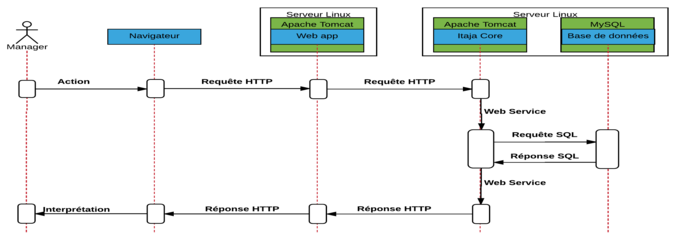
\includegraphics[scale=0.7]{images/diagrammeSequence.png}
		  \caption{Diagramme de séquences}
		\end{center}
	  \end{figure}
	  
      \section{Le diagramme de déploiement}
      Le diagramme de déploiement nous permettra de représenter l'utilisation de l'infrastructure physique par le système et la manière dont les composants du système sont répartis ainsi que leurs relations entre eux.
      
	\begin{figure}[H]
		\begin{center}
		  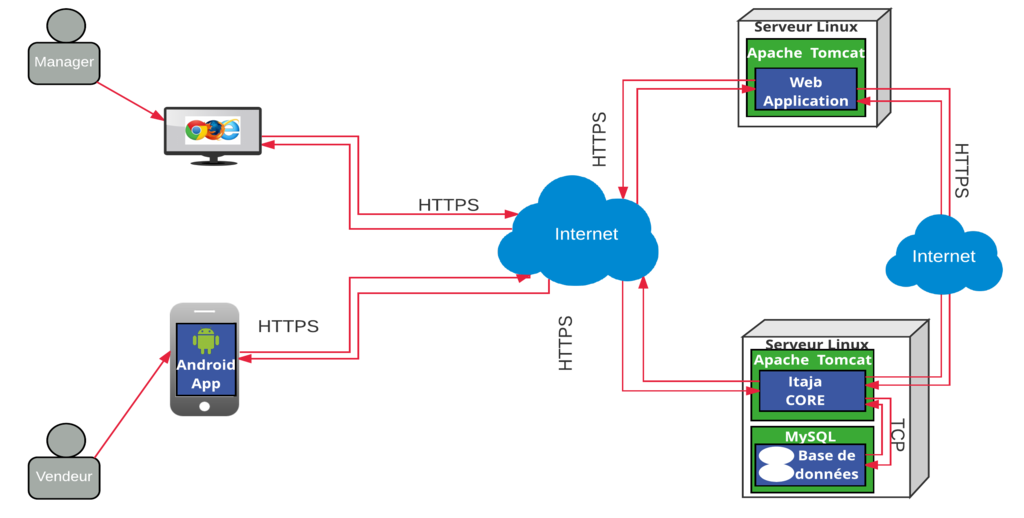
\includegraphics[scale=0.3]{images/diagrammeDeployement.png}
		  \caption{Diagramme de déploiement}
		\end{center}
	  \end{figure}

    \chapter{Conception et réalisation}
      \section{Introduction}
	La conception de logiciel met en œuvre un ensemble d'activités qui, à partir d'une demande d'informatisation d'un processus permettent la conception, l'écriture et la mise au point d'un logiciel jusqu'à sa livraison au demandeur. Ce chapitre nous permettra de décrire \textbf{comment} nous allons réaliser l'application et avec quelles \textbf{technologies}.
	
      \section{Architecture Orientée Service}
	  \paragraph{}
	    \textbf{\gls{SOA}} est une forme d'architecture de médiation qui est un modèle d'interaction applicative qui met en œuvre des services (composants logiciels) avec une forte cohérence interne (par l'utilisation d'un format d'échange pivot, XML ou JSON) et avec des couplages externes (par l'utilisation d'une couche d'interface interopérable, le plus souvent un service web).
	    \\Une architecture orientée service se conforme à divers principes de gestion des services influençant directement le comportement intrinsèque d’une solution logicielle et le style de sa conception :
	      \begin{itemize}
		\item L’encapsulation des services.
		\item Le faible couplage des services avec la maintenance d’une relation réduisant les dépendances.
		\item Le contrat de service adhérent à un accord de communication, collectivement défini avec un ou plusieurs documents de description.
		\item L’abstraction des services dissimulant la logique du service à l’extérieur.
		\item La réutilisation des services partageant la logique entre plusieurs services avec l’intention de promouvoir la réutilisation.
		\item La composition des services.
		\item L’autonomie des services.
		\item L’optimisation des services.
		\item La découverte des services depuis leur description extérieure.
	      \end{itemize}
	      L’architecture orientée service représente un moyen technique d’intégration des divers systèmes d’information de l’entreprise considérant chaque ressource informatique comme un service.
	      
	      \paragraph{}
		La notion d’\textbf{interface} est importante dans l’approche orientée service. En effet, elle représente le point d’entrée unique vers les fonctionnalités de la solution logicielle et assure la communication grâce à l’échange de messages. Chaque message est porteur de la sémantique particulière à la solution logicielle. De plus ce message est rédigé dans un langage compréhensible aux deux parties en présence. Les services proposés d’une architecture agile décrivent la structure des messages qu’ils attendent du client.
		\\Le \textbf{service} est un composant clef de l'architecture orientée services. Il consiste en une fonction ou fonctionnalité bien définie. C'est aussi un composant autonome qui ne dépend d’aucun contexte ou service externe. Il est divisé en opérations qui constituent autant d'actions spécifiques que le service peut réaliser. On peut faire un parallèle entre opérations et services d'une part, et méthodes et classes dans le mode orienté objet d'autre part.

	  \begin{figure}[H]
	    \begin{center}
	      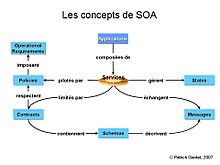
\includegraphics[scale=0.6, width=10cm]{images/soa.JPG}
	      \caption{Service Oriented Architecture (SOA)}
	    \end{center}
	  \end{figure}
      
      \section{Technologies utilisées}
	Pour arriver à réaliser la plate-forme, nous avons fait appel à plusieurs technologies selon les besoins. Nous détaillerons les \textbf{serveurs}, les \textbf{frameworks} avant de spécifier les \textbf{langages} informatiques qui vont avec ces derniers.
	
	\subsection{Apache Tomcat}
	  \textbf{Tomcat} est un serveur HTTP qui gère les servlets et les \gls{JSP}. Il nous a été d'une double utilité pour notre projet :
	  \begin{itemize}
	    \item c'est l'environnement où a été déployé \textbf{Itaja Core}, la couche de l'application qui contient les WebServices chargés de communiquer avec la base de données;
	    \item c'est également l'environnement où a été déployé la version compilée de l'application permettant l'accès depuis n'importe qual navigateur web
	  \end{itemize}
	  
	   \begin{figure}[H]
	      \begin{center}
		
\includegraphics[scale=0.6, width=4cm]{images/logoApacheTomcat.jpg}
		\caption{Logo de Bootstrap}
	      \end{center}
	    \end{figure}
	  
	\subsection{Angular}
	  \textbf{Angular} est un framework libre écrit en \gls{JS} par Google qui permet d'améliorer, au même titre que JQuery, la syntaxe de \gls{JS} et la productivité du développeur. Nous l'uitlisons parce qu'il est fondé sur l’extension du langage HTML par de nouvelles balises pour aboutir à une définition déclarative des pages web, par opposition à l’utilisation systématique de l’élément div​ et à la définition des éléments de présentation en JavaScript. Il permet au navigateur, une fois les données chargées, de ne plus avoir à se connecter au serveur avant la navigation entre les différentes pages de l'application.
	  
	  \begin{figure}[H]
	    \begin{center}
	      
\includegraphics[scale=0.6, width=3cm]{images/logoAngular.png}
	      \caption{Logo de Angular}
	    \end{center}
	  \end{figure}
	  
	  \subsection{TypeScript}
	    \textbf{TypeScript} est un langage de programmation libre et open source développé par Microsoft qui a pour but d'améliorer et de sécuriser la production de code JavaScript. Le code TypeScript est transcompilé en JavaScript, pouvant ainsi être interprété par n'importe quel navigateur web ou moteur JavaScript. Il est utilisé parce qu'il est typé et orienté objet; ce qui s'intègre dans un style général de programmation.
	    
	     \begin{figure}[H]
	      \begin{center}
		
\includegraphics[scale=0.6, width=3cm]{images/logoTypeScript.png}
		\caption{Logo de TypeScript}
	      \end{center}
	    \end{figure}
	    
	  \subsection{Bootstrap}
	    \textbf{Bootstrap} est une collection d'outils utile à la création du design (graphisme, animation et interactions avec la page dans le navigateur etc...) de sites et d'applications web. C'est un ensemble qui contient des codes HTML et CSS, des formulaires, boutons, outils de navigation et autres éléments interactifs, ainsi que des extensions JavaScript en option. Il a le mérite de donner de la beauté et du goût nos pages Webs.
	    
	    \begin{figure}[H]
	      \begin{center}
		
\includegraphics[scale=0.6, width=4cm]{images/logoBootstrap.png}
		\caption{Logo de Bootstrap}
	      \end{center}
	    \end{figure}
	  
	  \section{Environnement technique}
	  \subsection{Méthodologie : Agile - SCRUM}
	    \textbf{Agile} est une méthode de développement informatique permettant de concevoir des logiciels en impliquant au maximum le client, ce qui permet une grande réactivité à ses demandes. Elles visent la satisfaction réelle du besoin du client, et non d'un contrat établi préalablement.
	    \\\textbf{Scrum} est un schéma d’organisation qui s’axe autour de petits sprints durant lesquels l’équipe arrive à développer des produits complexes tout en enchaînant les tâches quotidiennes. Pour accompagner les sprints, l’équipe se doit de suivre quelques rituels à savoir des réunions de planification de projet, des rétrospectives de ce qui a été fait ou non, etc.).
	    \\Dans le cadre de notre projet, nous avons fait des sprints de une semaine chacun et organisons les réunions chaque matin à une heure convenue (9h).
	 
	  \subsection{Outils projet}
	    \begin{itemize}
	      \item[\ding{42}] \textbf{G Suite}\\
		\textbf{G Suite} est une suite d'outils et de logiciels de productivité de type Cloud computing et de groupware destinée aux professionnels, proposée par Google sous la forme d'un abonnement.
		\\La suite inclut les applications Web de Google les plus courantes, comme \textbf{Gmail, Google Hangouts, Google Agenda, Google+, Google Drive, Google Docs, Sheets, Slides et Forms et Google Sites}. Elle inclut aussi des fonctionnalités répondant aux besoins des entreprises, comme les adresses de courrier électronique personnalisées, un espace de stockage de 30 Go pour les documents et les e-mails, ainsi qu'une assistance 24h/24, 7j/7 par téléphone et par messagerie électronique.

	      \item[\ding{42}] \textbf{Jira}\\
		\textbf{Jira} est un système de suivi de bugs, de gestion des incidents, et de gestion de projets développé par Atlassian. Les fonctions qu'offrent Jira et pour lesquelles nous l'avons utilisé sont:
		\begin{itemize}
		  \item[•] \textbf{Planification} : Jira nous permet de créer des user stories et des tickets, de planifier des sprints et d'affecter les tâches à l'ensemble de l'équipe de développement.
		  \item[•] \textbf{Suivi} : Jira nous permet de définir des priorités et de bénéficier d'une visibilité totale pour discuter du travail de l'équipe dans son contexte.
		  \item[•] \textbf{Génération des rapports} : Jira améliore les performances de l'équipe en exploitant en temps réel les données visuelles des rapports.
		\end{itemize}
     
	      \item[\ding{42}] \textbf{Slack}\\
		\textbf{Slack} est une plateforme qui centralise les flux de communication. C'est un espace de travail numérique qui s'est placé au cœur de l'organisation et qui, en interconnectant toutes ses ressources (humaines ou techniques), nous permet de faire des gains de productivité. Une équipe Slack se compose des personnes suivantes :
		\begin{itemize}
		  \item Le propriétaire de l'équipe
		  \item Les administrateurs
		  \item Les collaborateurs
		  \item Les invités
		\end{itemize}
	  \end{itemize}
	  
	  \subsection{Intégration continue : Jenkins}
	    \textbf{Jenkins} est un outil open source d'intégration continue, écrit en Java, et qui fonctionne dans un conteneur de servlets tel qu’Apache Tomcat, ou en mode autonome avec son propre serveur Web embarqué. Les fonctions qu'offrent Jenkins et pour lesquelles nous l'avons utilisé sont:
		\begin{itemize}
		  \item[•] \textbf{Centralisation} : Jenkins permet à l'équipe de bénéficier d'informations communes.
		  \item[•] \textbf{Automatisation} : Jenkins permet d'effectuer l'ensemble des phases de productions (compilation, tests, 	déploiement...) sans ou avec très peu d'intervention humaine.
		  \item[•] \textbf{Historisation} : Jenkins permet de garder les productions précédentes et de voir l'évolution des productions.
		\end{itemize}
	    
	  \subsection{Gestionnaire de code source : Bitbucket avec le Git}
	  \textbf{Bitbucket} est un outil qui nous a permi de stocker l'ensemble des fichiers de notre projet tout en conservant la chronologie de toutes les modifications qui ont été effectuées dessus. Il permet notamment de retrouver les différentes versions d'un lot de fichiers connexes et de servir de repo source à l'intégration continue par Jenkins.
	  
      \section{Réalisation}
	Pour cette section, nous avons choisi de présenter trois captures d'écran de l'application. Vous trouverez une large gamme des captures d'écran dans l'annexe.
	\subsection{Capture de la page du dashboard}
	\begin{figure}[H]
	\begin{center}
	\includegraphics[scale=1, width=18cm]{images/login.png}
	\caption{Page de connexion}
	\end{center}
	\end{figure}
\subsection{Capture de création de cours }
\begin{figure}[H]
\begin{center}
\includegraphics[scale=1, width=18cm]{images/cours_1.png}
\caption{Page de création de cours}
\end{center}
\end{figure}
%%conclusion
\lhead[]{} \rhead[]{} \chead[]{}
\conclusion
Le présent travail de fin de formation intitulé : <<Conception et réalisation d'une plate-forme de gestion d'emplois du temps universitaire : cas de l'Université d'Abomey-Calavi (UAC)>> nous a permis de proposer une solution pour gérer les emplois du temps au sein du \gls{SGETPOIP} de l'\gls{UAC}.
Eu regard à notre sujet, nous nous sommes posé quelques questions ?
\begin{itemize}
\item[•] Comment proposer une solution opérationnelle pour aider le \gls{SGETPOIP}
\item[•] Quelles technologies choisir pour résoudre le problème
\item[•] Comment réduire le fossé (en terme de gestion d'emplois du temps) qui existe entre écoles et facultés
\end{itemize}
Sur ce, la mise en oeuvre d'une application Web pour la gestion d'emplois du temps a été le choix determinant pour résoudre tous les problèmes ci-haut.
Au cours de ce travail nous avons présenté les différentes étapes de la conception avec le puissant outil de modélisation \gls{UML} ainsi que la réalisation de l'application avec le Framework \gls{PHP} le plus populaire \textbf{Symfony}. S'il faut préciser quelque chose, ce projet nous a permis d'approfondir nos connaissances dans le domaine du développement Web.
\paragraph{}
Aussi, grâce à cette application la publication d'emplois du temps, leur gestion ainsi que le suivi des cours deviennent possibles et faciles.
\paragraph{}
Aux lecteurs de ce document, nous rappelons que cette application est loin d'avoir la prétention d'être parfaite. Elle n'est qu'une proposition de solutions aux problèmes de gestion d'emplois du temps universitaire. Nous restons ouvert aux critiques et suggestions.
\paragraph{}



%%biblio
\newpage
\begin{thebibliography}{9}
\addcontentsline{toc}{chapter}{Bibliographie}

   \bibitem{IUPM}
          Jebsoubo Frederic, Ndiguissem Rodrigue
          \emph{\LaTeX: Création d’une application Web pour la gestion d'emplois de temps et les suivis des cours : cas de l’Institut Universitaire Polytechnique de Mongo (IUPM-Tchad), }
          Année académique : 2014-2015, p57.
          
   \bibitem{UAC}
          Dr. Ir. Sylvain KPENAVOUN CHOGOU,
          \emph{Données statistiques provisoires de l’année académique 2014-2015 }.
          2016.  
               
   \bibitem{UAC_Wiki}
          \url{https://fr.wikipedia.org/wiki/Universit%C3%A9_d%27Abomey-Calavi}
          \emph{du 05 août 2016}

   \bibitem{ib}
		\url{http://www.ib-formation.fr/catalogue/nbs-details/catref/universib-gouvernance-informatique-gestion-de-projets-et-methodes-conduite-de-projets/ref/mg722/realiser-lanalyse-fonctionnelle-et-technique-dun-projet-informatique, }
		\emph{du 17 juillet 2016}
	
	\bibitem{uml}
          Carina ROELS,
          \emph{Débutez l'analyse logicielle avec UML}.
          \url{https://openclassrooms.com/courses/debutez-l-analyse-logicielle-avec-uml}
          OpenClassrooms,
          \emph{du 15 avril 2016}
	
	\bibitem{wiki1}
          \url{https://fr.wikipedia.org/wiki/Conception_de_logiciel}
          Wikipedia,
          \emph{du 17 juillet 2016}
	
	\bibitem{symfony}
          Alexandre BACCO,
          \emph{Développez votre site web avec le framework Symfony}.
          \url{https://openclassrooms.com/courses/developpez-votre-site-web-avec-le-framework-symfony}
          OpenClassrooms,
          \emph{du 17 juillet 2016}
	
	\bibitem{wiki2}
          \url{https://fr.wikipedia.org/wiki/Hypertext_Markup_Language}
          Wikipedia,
          \emph{du 14 juillet 2016}
	
\end{thebibliography}


%

\appendix
\chapter{Annexe 1}
\begin{figure}[H]
\begin{center}
	\includegraphics[scale=1, width=18cm]{images/dash.png}
	\caption{Résultat de recherche d'un cours}
\end{center}
\end{figure}

\begin{figure}[H]
\begin{center}
	\includegraphics[scale=1, width=18cm]{images/cours_1.png}
	\caption{Ajout de cours (Date, Heure début et Heure fin)}
\end{center}
\end{figure}

\begin{figure}[H]
\begin{center}
	\includegraphics[scale=1, width=18cm]{images/cours_2.png}
	\caption{Ajout de cours (Salle)}
\end{center}
\end{figure}

\begin{figure}[H]
\begin{center}
	\includegraphics[scale=1, width=18cm]{images/cours_3.png}
	\caption{Ajout de cours (Enseignant)}
\end{center}
\end{figure}

\begin{figure}[H]
\begin{center}
	\includegraphics[scale=1, width=18cm]{images/cours_4.png}
	\caption{Ajout d'un cours (Matière, Formation et Observations)}
\end{center}
\end{figure}

\begin{figure}[H]
\begin{center}
	\includegraphics[scale=1, width=18cm]{images/liste_batiment.png}
	\caption{Liste des bâtiments}
\end{center}
\end{figure}

\begin{figure}[H]
\begin{center}
	\includegraphics[scale=1, width=18cm]{images/liste_salle.png}
	\caption{Liste de la disponibilité des enseignants}
\end{center}
\end{figure}

\begin{figure}[H]
\begin{center}
	\includegraphics[scale=1, width=18cm]{images/recherche.png}
	\caption{Page de recherche}
\end{center}
\end{figure}

\begin{figure}[H]
\begin{center}
	\includegraphics[scale=1, width=18cm]{images/liste_disponibilite.png}
	\caption{Liste des disponibilités des salles}
\end{center}
\end{figure}

\begin{figure}[H]
\begin{center}
	\includegraphics[scale=1, width=18cm]{images/liste_cours.png}
	\caption{Liste des cours}
\end{center}
\end{figure}
\end{document}